%% The following is a directive for TeXShop to indicate the main file
%%!TEX root = diss.tex

\chapter{Introduction}
\label{ch:Introduction}

Elastic materials are ubiquitous in everyday life. Many objects we
interact with are organic in nature such as plants, animals, food, and
most importantly our own bodies. Interestingly, most organic solids
are nearly incompressible (due to their high water content), which
makes them particularly difficult to simulate. Human soft tissue, for
instance, is essentially incompressible, with a Poisson's ratio close
to 0.5 \cite{fung2013biomechanics}. As a result, much of contemporary
research in computer graphics focuses on robust simulation of
incompressible hyperelastic solids (see Sec.~\ref{sec:related}). We
focus on the popular Neo-Hookean models, which are relatively simple
while including non-linearity and the temptation to control
incompressibility by setting Poisson's ratio $\nu \simeq 0.5$.

% Unfortunately, this approach for soft tissue simulation enforces
% incompressibility indirectly with a per-element energy term, which
% means that the material parameters like Poisson's ratio are
% dependent on the resolution of the simulation mesh. In addition,
% high Poisson's ratios cause numerical instability and locking when
% coupled with a coarse discretization \cite{Irving:2007}.

However, it is impossible to emulate true incompressibility and
extremely difficult to simulate even near-incompressibility with this
approach.  This is because as the material approaches
incompressibility $\nu \rightarrow 0.5$, the first Lam\'e parameter
% (which penalizes volume change)
$\lambda \rightarrow +\infty$ (see Sec.~\ref{sec:back} for
background). The numerical and visual artifacts arising from the failure
to correctly enforce incompressibility is known as {\em locking.}

There are multiple aspects of locking which are problematic for
simulating volume preserving elastic solids.  First, high Poisson's
ratios make the system stiff, which results in stiffness related
issues such as stability, and artificial damping.  Somewhat related to
this, when using linear tetrahedral elements and element-wise volume
constraints, the resulting system becomes highly overconstrained.
Another aspect
% is volumetric locking, which
arises from the choice of the constitutive equation, where volumetric
stress depends on $\lambda$.  In classical FEM theory, C\'ea's Lemma
dictates that the quasi-best approximation error depends not only on
mesh discretization error, but also on $\lambda$. Hence, when
$\lambda \rightarrow +\infty$, the finite element solution cannot be a
reliable predictor of the solution of the PDE. A more detailed
explanation can be found in \cite{Braess:2007}.

There are multiple approaches to tackle this issue: the simplest being
just using higher-order elements or hexahedral elements. However, the
increased computational cost and difficulty of implementation might
not be desirable. Another class of popular methods is non-conforming
finite elements (such as the Discontinous Galerkin class of methods),
where the additional or non-conforming degrees of freedom allow
significant deformation and therefore reduce the stiffness of the
system.  The last approach includes methods that seek to remove these
element-wise constraints through Mixed Finite Elements or coarsened
constraints, both of which are related to our method.

Our core idea is to tease apart the concept of {\em
	incompressibility}, a constraint on a derivative (the deformation
gradient) from the related concept of {\em volume preservation}, a
constraint on an integral (the volume of a finite region of material
that we call a ``zone''). Incompressibility is enforced per element in
the standard Neo-Hookean models, usually implicitly, using an energy
term. By contrast, we enforce volume preservation as an explicit
constraint on the volume of a zone. Volume preservation gives us
considerable flexibility to choose larger zones that span multiple
elements, zones that are independent of discretization, and zones that
are aligned with meaningful anatomical tissue compartments (muscles,
abdomen, breast, etc.). Zones may also overlap (e.g., we can preserve
both the total volume of a body, and volumes of important tissue
compartments).

A second key idea is that since volume preservation is already
enforced using constraints, we can use much smaller values of
$\lambda$ or $\nu$, thereby avoiding locking and related numerical
instabilities. This can, of course, lead to volume loss per element
but that will be compensated by volume gain in other elements in a
zone to preserve volume. In other words, our simulation mesh may be
viewed as a type of Arbitrary Lagrangian-Eulerian (ALE) mesh, in which
volume is never lost but allowed to flow from one cell to another. To
our knowledge, this technique has not yet been closely studied with
FEM simulations in computer graphics.

Note that $\lambda$ now controls only element volume, rather than the
incompressibility of the material. In the rest of the paper we will
repurpose the first Lam\'e parameter $\lambda$ to control volume
change \emph{per element}, instead of \emph{zonal} volume change.
% TODO shall we skip the hat? and just use Lambda?
% For greater clarity, we will denote this {\em element Lam\'e}
% parameter as $\hat{\lambda}$, but
We will continue to use the term Poisson's ratio ($\nu$) in the
classical sense.

Large deformations, especially with moving Dirichlet boundary
conditions and contact, may produce severely degenerate (even
inverted) elements, and break traditional energy models. This issue
has attracted much attention in the community \cite{Irving:2007,
	Stomakhin:2012,Smith:2018}.  While our $\lambda$ values are no
longer constrained by volume preservation, there is still a need to
penalize extreme volume loss per element to avoid such degeneracies.
We address this in Sec.~\ref{sec:penalty} with an amendment to the
volume penalty term found in compressible elastic energy
models. Additionally, the proposed correction improves the compression
response in invertible energies.
%Compared to the Stable Neo-Hookean
%model \cite{Smith:2018}, our penalty method stays faithful to the
%classical Neo-Hookean compression penalty, while providing reliable
%inversion recovery during extreme
%compression.% \todo{Add note about comparison with Stomakhin}

Human bodies are covered by a layer of skin, a complex multi-layered structure. The outer layer comprising the epidermis is much stiffer than the underlying tissues, and significantly affects the quality of deformation. We propose a simple model of the epidermis and show that this
extension contributes heavily to the appearance of realistic tissue deformation.


A simple illustration of these ideas is given in
Figure~\ref{fig:twotets}. It illustrates the more general scenario in
which locking artifacts increase at lower mesh resolutions, whereas our
volume preservation is independent of the discretization of the zones.


% there
% are two tetrahedral elements connected at one triangle face; one
% element is flattened, while the other is allowed to deform. When
% compression is penalized locally on each element, the total volume of
% the system will never be preserved, and so the two element system will
% necessarily lose volume. 

% In the context of computer graphics, we are most interested in
% conserving the aesthetic properties visible on the surface of the
% solid.  With this in mind, we propose to constrain the volume of the
% solid zonally, and relax the Poisson's ratio of the material. This
% allows volume in the same zone to flow from one element to another,
% which removes locking artifacts.  This technique turns the purely
% Lagrangian approach to FEM simulations into an arbitrary
% Lagrangian-Eulerian formulation (ALE) because the FEM mesh becomes
% loosely coupled to the solid material.  

% DKP This could be moved to Results
Figure~\ref{fig:teaser} shows the practical relevance of good volume
preservation.  Closeups of the belly (yellow boxes) and side waist in
front view (red boxes) depict tissue displacement in false color, and
yield more insights. We see that the traditional Unconstrained
Neo-Hookean (UNH) model compresses under the waistband by losing volume,
without significantly extruding tissue away (e,h), whereas our method
extrudes tissue more realistically, producing a sharp bulge (g,j) due to
volume preservation.  Increasing $\nu$ doesn't help the UNH models since
locking reduces the deformation (f,i).

{\em Contributions:} we propose a new approach for simulating human
tissues and other soft objects that preserve volume, while avoiding
the common pitfalls of standard incompressible elasticity models. In
addition to avoiding locking artifacts, our zonal volume constraint
formulation makes deformation independent of discretization, and
allows zones to be aligned with meaningful anatomical tissue
compartments.  In addition, we repurpose the first Lam\'e parameter to
support inversion robustness and introduce a new form of the
compression penalty.  We also extend the elastic energy potential to
model the stiff epidermis, and demonstrate its importance.  Finally,
we propose a simple but complete pipeline for assigning volumetric
zones using weights on the surface of the volumetric mesh, and
demonstrate the application of these methods to predicting the fit of
tight fitting garments.

\begin{figure}[tb]
	\centering
	\begin{subfigure}{.32\linewidth}
		\centering
		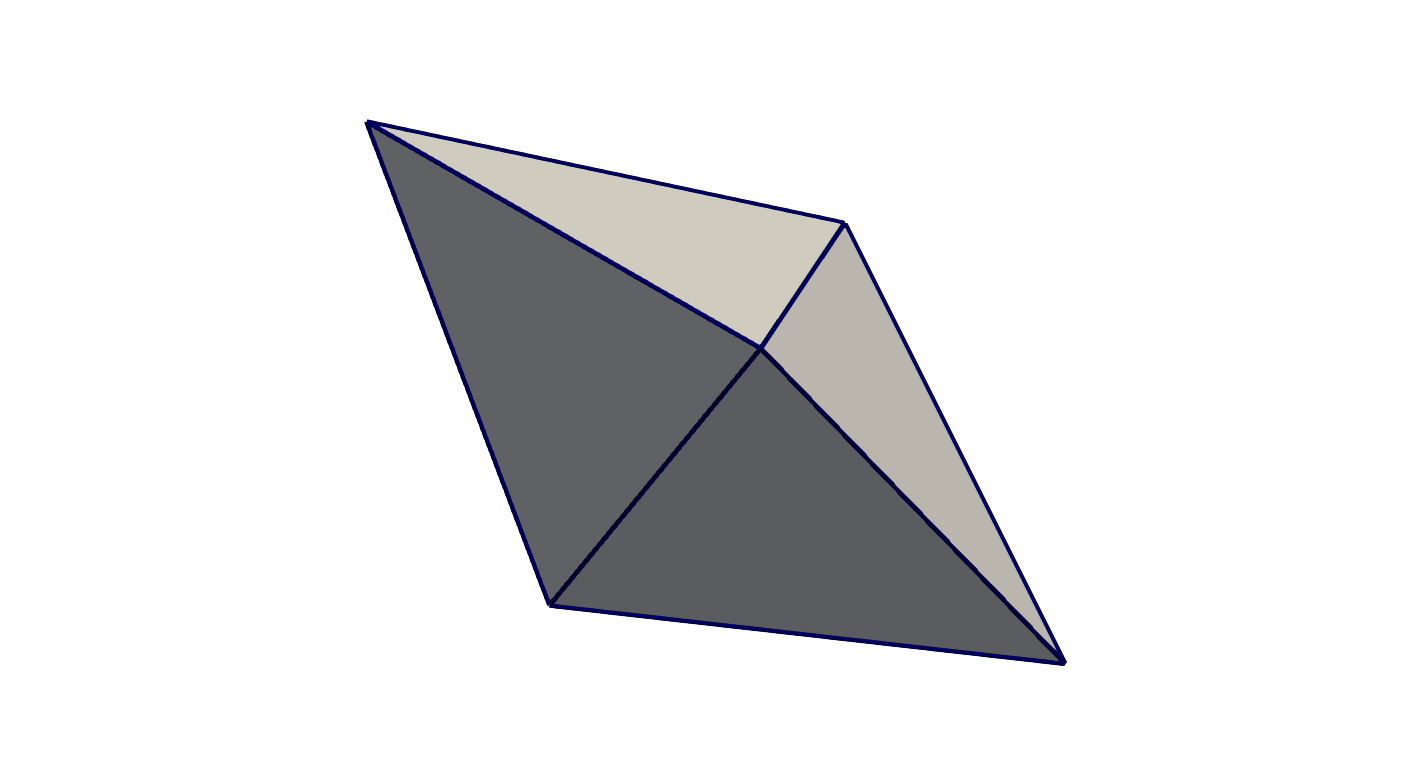
\includegraphics[width=1.0\textwidth]{images/simple_ref.png}
		\caption*{(a)}
		\label{sfig:simple_ref}
	\end{subfigure}%
	\begin{subfigure}{.32\linewidth}
		\centering
		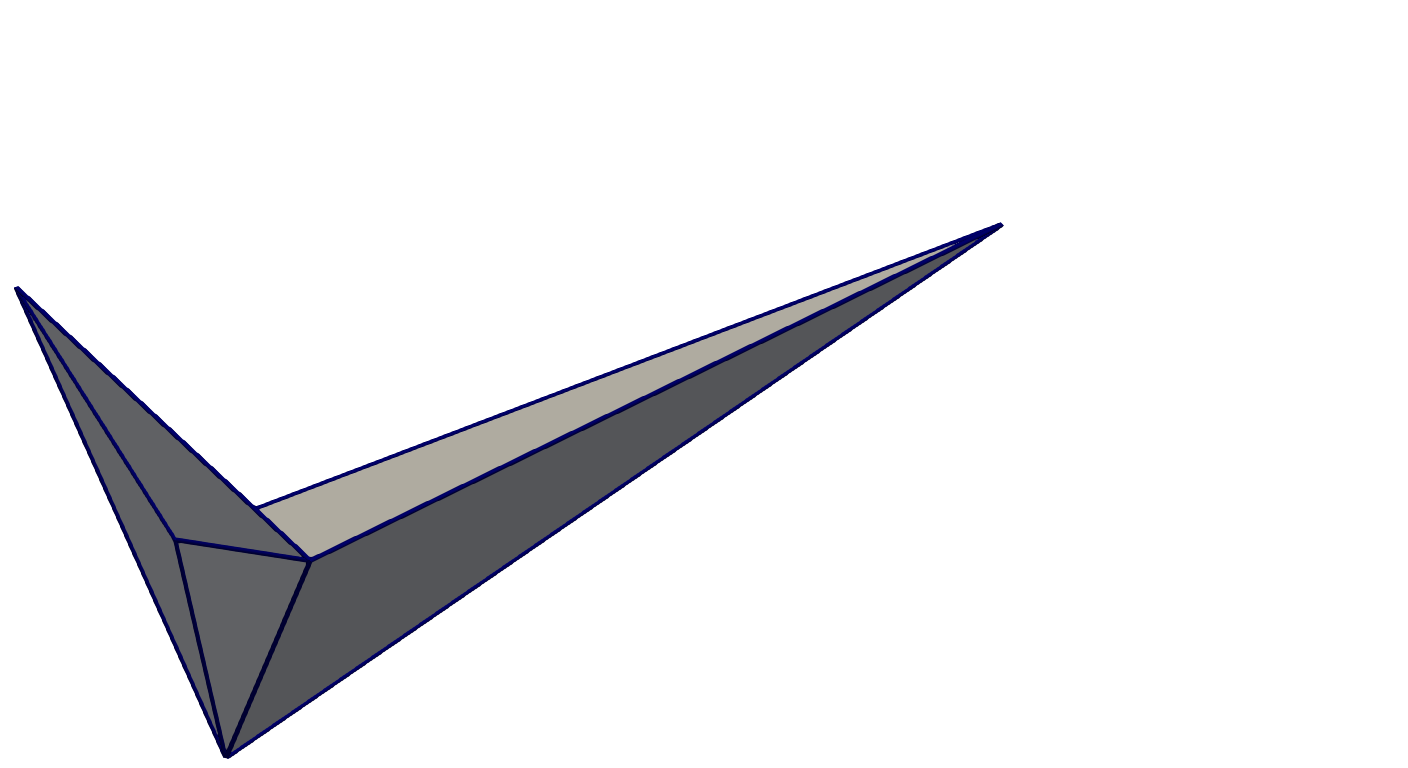
\includegraphics[width=1.0\textwidth]{images/simple.png}
		\caption*{(b)}
		\label{sfig:simple}
	\end{subfigure}%
	\begin{subfigure}{.32\linewidth}
		\centering
		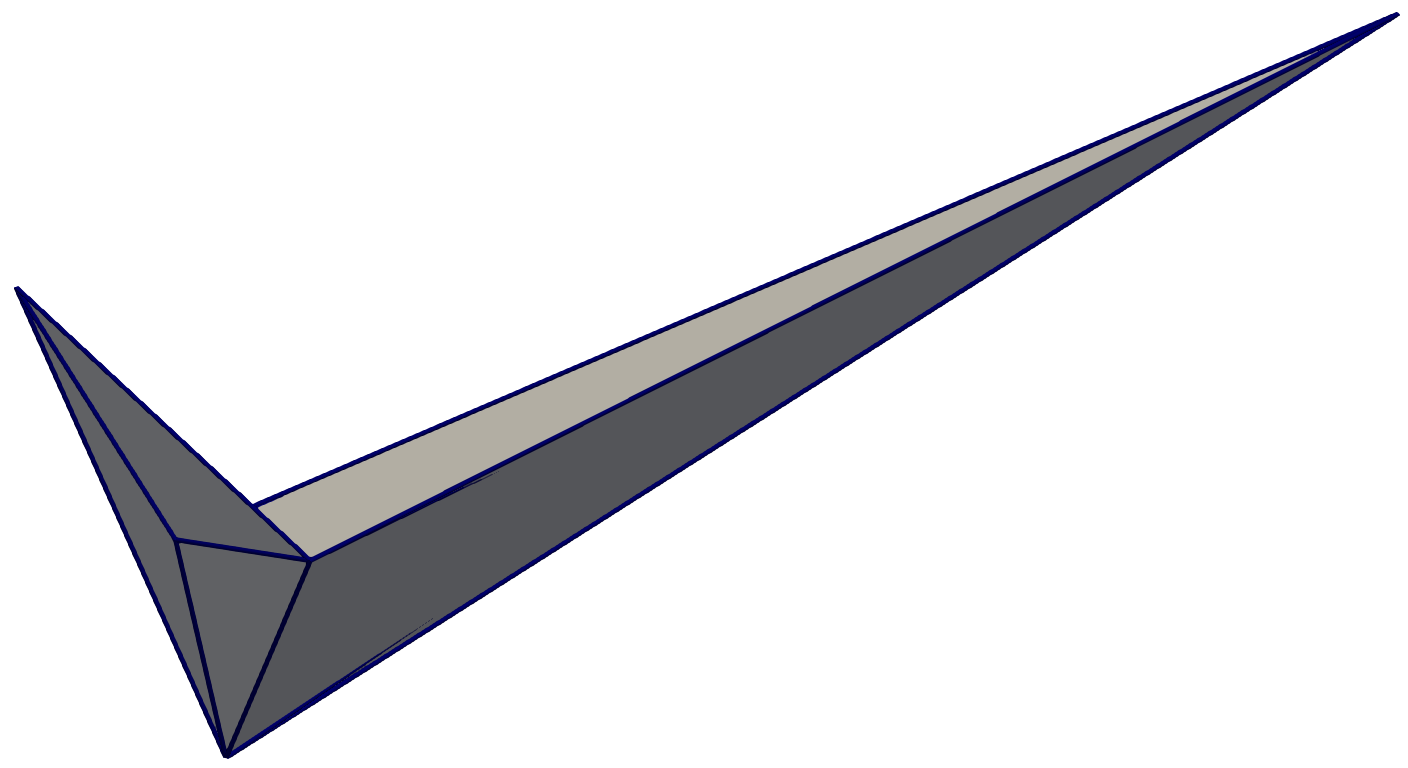
\includegraphics[width=1.0\textwidth]{images/simple_vc.png}
		\caption*{(c)}
		\label{sfig:simple_vc}
	\end{subfigure}%
	\caption{\textbf{Two Tet Simulation}: (a) The reference state of the mesh, where two
		tetrahedrons of equal volume are joined together by a face. The left tetrahedron is constrained
		by Dirichlet boundary conditions to be compressed into a plane. (b) With an unconstrained Neo-Hookean (UNH) model Without the
		volume constraint, the total volume of the final mesh is $46.628\%$ of the original. (c) With a volume constraint (CNH model), the tetrahedron on the righ inflates to twice
		the volume to keep the total volume constant.
	}
	\label{fig:twotets}
\end{figure} 

